\documentclass[twoside]{book}

% Packages required by doxygen
\usepackage{fixltx2e}
\usepackage{calc}
\usepackage{doxygen}
\usepackage{graphicx}
\usepackage[utf8]{inputenc}
\usepackage{makeidx}
\usepackage{multicol}
\usepackage{multirow}
\PassOptionsToPackage{warn}{textcomp}
\usepackage{textcomp}
\usepackage[nointegrals]{wasysym}
\usepackage[table]{xcolor}

% Font selection
\usepackage[T1]{fontenc}
\usepackage{mathptmx}
\usepackage[scaled=.90]{helvet}
\usepackage{courier}
\usepackage{amssymb}
\usepackage{sectsty}
\renewcommand{\familydefault}{\sfdefault}
\allsectionsfont{%
  \fontseries{bc}\selectfont%
  \color{darkgray}%
}
\renewcommand{\DoxyLabelFont}{%
  \fontseries{bc}\selectfont%
  \color{darkgray}%
}
\newcommand{\+}{\discretionary{\mbox{\scriptsize$\hookleftarrow$}}{}{}}

% Page & text layout
\usepackage{geometry}
\geometry{%
  a4paper,%
  top=2.5cm,%
  bottom=2.5cm,%
  left=2.5cm,%
  right=2.5cm%
}
\tolerance=750
\hfuzz=15pt
\hbadness=750
\setlength{\emergencystretch}{15pt}
\setlength{\parindent}{0cm}
\setlength{\parskip}{0.2cm}
\makeatletter
\renewcommand{\paragraph}{%
  \@startsection{paragraph}{4}{0ex}{-1.0ex}{1.0ex}{%
    \normalfont\normalsize\bfseries\SS@parafont%
  }%
}
\renewcommand{\subparagraph}{%
  \@startsection{subparagraph}{5}{0ex}{-1.0ex}{1.0ex}{%
    \normalfont\normalsize\bfseries\SS@subparafont%
  }%
}
\makeatother

% Headers & footers
\usepackage{fancyhdr}
\pagestyle{fancyplain}
\fancyhead[LE]{\fancyplain{}{\bfseries\thepage}}
\fancyhead[CE]{\fancyplain{}{}}
\fancyhead[RE]{\fancyplain{}{\bfseries\leftmark}}
\fancyhead[LO]{\fancyplain{}{\bfseries\rightmark}}
\fancyhead[CO]{\fancyplain{}{}}
\fancyhead[RO]{\fancyplain{}{\bfseries\thepage}}
\fancyfoot[LE]{\fancyplain{}{}}
\fancyfoot[CE]{\fancyplain{}{}}
\fancyfoot[RE]{\fancyplain{}{\bfseries\scriptsize Generated on Sat Jun 30 2018 23\+:26\+:22 for Trabalho Final C\+G by Doxygen }}
\fancyfoot[LO]{\fancyplain{}{\bfseries\scriptsize Generated on Sat Jun 30 2018 23\+:26\+:22 for Trabalho Final C\+G by Doxygen }}
\fancyfoot[CO]{\fancyplain{}{}}
\fancyfoot[RO]{\fancyplain{}{}}
\renewcommand{\footrulewidth}{0.4pt}
\renewcommand{\chaptermark}[1]{%
  \markboth{#1}{}%
}
\renewcommand{\sectionmark}[1]{%
  \markright{\thesection\ #1}%
}

% Indices & bibliography
\usepackage{natbib}
\usepackage[titles]{tocloft}
\setcounter{tocdepth}{3}
\setcounter{secnumdepth}{5}
\makeindex

% Hyperlinks (required, but should be loaded last)
\usepackage{ifpdf}
\ifpdf
  \usepackage[pdftex,pagebackref=true]{hyperref}
\else
  \usepackage[ps2pdf,pagebackref=true]{hyperref}
\fi
\hypersetup{%
  colorlinks=true,%
  linkcolor=blue,%
  citecolor=blue,%
  unicode%
}

% Custom commands
\newcommand{\clearemptydoublepage}{%
  \newpage{\pagestyle{empty}\cleardoublepage}%
}


%===== C O N T E N T S =====

\begin{document}

% Titlepage & ToC
\hypersetup{pageanchor=false,
             bookmarks=true,
             bookmarksnumbered=true,
             pdfencoding=unicode
            }
\pagenumbering{roman}
\begin{titlepage}
\vspace*{7cm}
\begin{center}%
{\Large Trabalho Final C\+G }\\
\vspace*{1cm}
{\large Generated by Doxygen 1.8.7}\\
\vspace*{0.5cm}
{\small Sat Jun 30 2018 23:26:22}\\
\end{center}
\end{titlepage}
\clearemptydoublepage
\tableofcontents
\clearemptydoublepage
\pagenumbering{arabic}
\hypersetup{pageanchor=true}

%--- Begin generated contents ---
\chapter{Aplicação Bezier}
\label{index}\hypertarget{index}{}\begin{DoxyAuthor}{Author}
Grupo (ordem alfabética)\+: Igor, Nathália \& Yves
\end{DoxyAuthor}
\begin{DoxyDate}{Date}
30/08/2018
\end{DoxyDate}
Esse trabalho procura ilustrar superficies de Bezier através de 4 retalhos diferentes (um de cada vez).

Usabilidade\+: Os comandos são controlados via teclado. Segue sua lista\+:

Controle da resolução do retalho\+:
\begin{DoxyItemize}
\item Ao pressionar a tecla \char`\"{}\+U\char`\"{} (maiúsculo), a quantidade de amostras na direção U aumenta.
\item Ao pressionar a tecla \char`\"{}u\char`\"{} (minúsculo), a quantidade de amostras na direção U diminui.
\item Ao pressionar a tecla \char`\"{}\+V\char`\"{} (maiúsculo), a quantidade de amostras na direção V aumenta.
\item Ao pressionar a tecla \char`\"{}v\char`\"{} (minúsculo), a quantidade de amostras na direção U diminui.
\end{DoxyItemize}

Controle de animação (rotação)\+:
\begin{DoxyItemize}
\item Pressione tecla \char`\"{}a\char`\"{} para ligar/desligar rotação.
\item Pressione tecla \char`\"{}s\char`\"{} para movimento um passo de cada vez (\char`\"{}camera lenta\char`\"{}).
\item As teclas \char`\"{}$<$-\/\char`\"{} e \char`\"{}-\/$>$\char`\"{} controlam a direção e velocidade da rotação no eixo y.
\item As teclas de seta (para cima e para baixo) controlam a direção e velocidade da rotação no eixo s.
\item Pressione tecla \char`\"{}r\char`\"{} para voltar ao esquema original de posição, antes de iniciar rotação.
\item Pressione \char`\"{}0\char`\"{} (número zero) para zerar a velocidade de rotação.
\end{DoxyItemize}

Zoom\+:
\begin{DoxyItemize}
\item Pressione tecla \char`\"{}z\char`\"{} para aumentar o zoom.
\item Pressione tecla \char`\"{}x\char`\"{} para diminuir o zoom.
\end{DoxyItemize}

Preenchimento e sombra\+:
\begin{DoxyItemize}
\item Ao pressionar a tecla \char`\"{}p\char`\"{}, alterne as opções de preenchimento da superfície (G\+L\+\_\+\+L\+I\+N\+E ou G\+L\+\_\+\+F\+I\+L\+L).
\item Ao pressionar a tecla \char`\"{}o\char`\"{}, alterne as opções de sombra (G\+L\+\_\+\+F\+L\+A\+T e G\+L\+\_\+\+S\+M\+O\+O\+T\+H).
\end{DoxyItemize}

Para rodar o programa basta digitar os seguintes comandos na linha de comando\+:

\begin{quote}
gcc -\/o Trabalho\+Final \hyperlink{TrabalhoFinal_8c}{Trabalho\+Final.\+c} -\/l\+G\+L -\/l\+G\+L\+U -\/lglut -\/lm \begin{quote}
./\+Trabalho\+Final \end{quote}
\end{quote}


O\+B\+S\+: O programa foi desenvolvido usando Open\+G\+L 3. 
\chapter{File Index}
\section{File List}
Here is a list of all documented files with brief descriptions\+:\begin{DoxyCompactList}
\item\contentsline{section}{\hyperlink{TrabalhoFinal_8c}{Trabalho\+Final.\+c} \\*Programa para ilustrar superficies de Bezier através de 4 retalhos diferentes (um de cada vez) }{\pageref{TrabalhoFinal_8c}}{}
\item\contentsline{section}{\hyperlink{TrabalhoFinal_8h}{Trabalho\+Final.\+h} \\*Declaração das funções para o programa Trabalho\+Final }{\pageref{TrabalhoFinal_8h}}{}
\end{DoxyCompactList}

\chapter{File Documentation}
\hypertarget{TrabalhoFinal_8c}{\section{Trabalho\+Final.\+c File Reference}
\label{TrabalhoFinal_8c}\index{Trabalho\+Final.\+c@{Trabalho\+Final.\+c}}
}


Programa para ilustrar superficies de Bezier através de 4 retalhos diferentes (um de cada vez).  


{\ttfamily \#include \char`\"{}Trabalho\+Final.\+h\char`\"{}}\\*
{\ttfamily \#include $<$stdlib.\+h$>$}\\*
{\ttfamily \#include $<$math.\+h$>$}\\*
{\ttfamily \#include $<$limits.\+h$>$}\\*
{\ttfamily \#include $<$G\+L/glut.\+h$>$}\\*
Include dependency graph for Trabalho\+Final.\+c\+:
\nopagebreak
\begin{figure}[H]
\begin{center}
\leavevmode
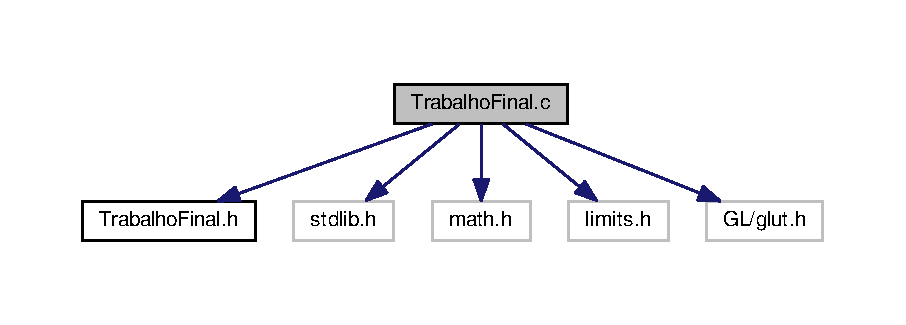
\includegraphics[width=350pt]{TrabalhoFinal_8c__incl}
\end{center}
\end{figure}
\subsection*{Functions}
\begin{DoxyCompactItemize}
\item 
void \hyperlink{TrabalhoFinal_8c_a38e4a81c795cc1492e2dbf4388dc2e03}{keyboard\+Func} (unsigned char key, int x, int y)
\begin{DoxyCompactList}\small\item\em Funcionalidades do teclado, onde todas as funcionalidades e animações do programa serão feitas pelo teclado. As funcionalidades estão listadas em detalha na página inical da documentação. \end{DoxyCompactList}\item 
void \hyperlink{TrabalhoFinal_8c_a503dca08df7da12b8659d41ed3fdf9fa}{rot\+Key\+Func} (int key, int x, int y)
\begin{DoxyCompactList}\small\item\em Trata as quatro possibilidades de movimentos rotacionais (cima,baixo,esquerda,direita). \end{DoxyCompactList}\item 
void \hyperlink{TrabalhoFinal_8c_aa0bf20c41c51e3378eff1bed8c8ad7e7}{Key\+Up} ()
\begin{DoxyCompactList}\small\item\em As quatro funções\+: Key\+Up, Key\+Down, Key\+Left e Key\+Right limitam a mudança de direção de rotação apenas com \char`\"{}reset\char`\"{}. \end{DoxyCompactList}\item 
void \hyperlink{TrabalhoFinal_8c_a67b12319ab360702a47400465268d886}{Key\+Down} ()
\begin{DoxyCompactList}\small\item\em As quatro funções\+: Key\+Up, Key\+Down, Key\+Left e Key\+Right limitam a mudança de direção de rotação apenas com \char`\"{}reset\char`\"{}. \end{DoxyCompactList}\item 
void \hyperlink{TrabalhoFinal_8c_a8feed104082b0773ee6a1e43dc62494a}{Key\+Left} ()
\begin{DoxyCompactList}\small\item\em As quatro funções\+: Key\+Up, Key\+Down, Key\+Left e Key\+Right limitam a mudança de direção de rotação apenas com \char`\"{}reset\char`\"{}. \end{DoxyCompactList}\item 
void \hyperlink{TrabalhoFinal_8c_a247cd4807e203e488d19c3e2d11d0dfe}{Key\+Right} ()
\begin{DoxyCompactList}\small\item\em As quatro funções\+: Key\+Up, Key\+Down, Key\+Left e Key\+Right limitam a mudança de direção de rotação apenas com \char`\"{}reset\char`\"{}. \end{DoxyCompactList}\item 
void \hyperlink{TrabalhoFinal_8c_a0a8efd509aaffafefd6d761748e3b688}{Reset\+Animation} ()
\begin{DoxyCompactList}\small\item\em Restaura posição original e define rotação igual a zero. \end{DoxyCompactList}\item 
void \hyperlink{TrabalhoFinal_8c_aaad754c5c3683cfa1ff97d2c381f7cf9}{Zero\+Rotation} ()
\begin{DoxyCompactList}\small\item\em Restaura posicao original e define rotação igual a zero. \end{DoxyCompactList}\item 
void \hyperlink{TrabalhoFinal_8c_acdf384c0ffd8a916ef177390d4231f20}{Shade\+Model\+Func} ()
\begin{DoxyCompactList}\small\item\em Sombra, alterna entre G\+L\+\_\+\+S\+M\+O\+O\+T\+H e G\+L\+\_\+\+F\+L\+A\+T. \end{DoxyCompactList}\item 
void \hyperlink{TrabalhoFinal_8c_a6d5b5815603b85d7b4c4cbcef41c9d04}{Fill\+Model\+Func} ()
\begin{DoxyCompactList}\small\item\em Preenchimento do poligono, alterna entre G\+L\+\_\+\+L\+I\+N\+E e G\+L\+\_\+\+F\+I\+L\+L. \end{DoxyCompactList}\item 
void \hyperlink{TrabalhoFinal_8c_a49231a37c9b57e3f5985645eea705aea}{Inc\+U} ()
\begin{DoxyCompactList}\small\item\em Incrementa \char`\"{}u\char`\"{}. \end{DoxyCompactList}\item 
void \hyperlink{TrabalhoFinal_8c_a9a94b4a40c2579e84929e96cd020fc76}{Dec\+U} ()
\begin{DoxyCompactList}\small\item\em Decrementa \char`\"{}u\char`\"{}. \end{DoxyCompactList}\item 
void \hyperlink{TrabalhoFinal_8c_a382fd47ad46d351c01316369a7a2a167}{Inc\+V} ()
\begin{DoxyCompactList}\small\item\em Incrementa \char`\"{}u\char`\"{}. \end{DoxyCompactList}\item 
void \hyperlink{TrabalhoFinal_8c_a243cc6a279207dca01da3d7e00f6a669}{Dec\+V} ()
\begin{DoxyCompactList}\small\item\em Decrementa \char`\"{}u\char`\"{}. \end{DoxyCompactList}\item 
void \hyperlink{TrabalhoFinal_8c_a5b0721aa50b4ff19c67311b6d8717635}{update\+Scene} (void)
\begin{DoxyCompactList}\small\item\em Desenha superfícies/retalhos com todas suas especificações. \end{DoxyCompactList}\item 
void \hyperlink{TrabalhoFinal_8c_a17a53fe9e683b81bdc7618f88b8b8502}{init\+Rendering} ()
\begin{DoxyCompactList}\small\item\em Inicializa Open\+G\+L (iluminação). \end{DoxyCompactList}\item 
void \hyperlink{TrabalhoFinal_8c_a5228d95579d96f983dea42fed8845620}{resize\+Window} (int w, int h)
\begin{DoxyCompactList}\small\item\em Efetua mudança nas dimensões da janela (aumentando ou diminuindo de acordo com ação do mouse). \end{DoxyCompactList}\end{DoxyCompactItemize}
\subsection*{Variables}
\begin{DoxyCompactItemize}
\item 
const float {\bfseries control\+Points} \mbox{[}4\mbox{]}\mbox{[}3\mbox{]}\mbox{[}4\mbox{]}
\item 
\hypertarget{TrabalhoFinal_8c_a87a33fdc879f0e3fef5d15e2804c3753}{G\+Lfloat {\bfseries zpos} = -\/6}\label{TrabalhoFinal_8c_a87a33fdc879f0e3fef5d15e2804c3753}

\item 
\hypertarget{TrabalhoFinal_8c_a93562df3836884e0dc63dbd95b75a4f8}{int {\bfseries Num\+U} = 4}\label{TrabalhoFinal_8c_a93562df3836884e0dc63dbd95b75a4f8}

\item 
\hypertarget{TrabalhoFinal_8c_a4814b2fc4eea75a00277521ca5b82dc4}{int {\bfseries Num\+V} = 4}\label{TrabalhoFinal_8c_a4814b2fc4eea75a00277521ca5b82dc4}

\item 
\hypertarget{TrabalhoFinal_8c_ab23abe23033bafbbdd760ff0001791c2}{const float {\bfseries P\+I2} = 2.\+0f$\ast$3.\+1415926535f}\label{TrabalhoFinal_8c_ab23abe23033bafbbdd760ff0001791c2}

\item 
\hypertarget{TrabalhoFinal_8c_aed3b8c4fc370319b45ddb3291e7efdeb}{G\+Lenum {\bfseries shade\+Model} = G\+L\+\_\+\+F\+L\+A\+T}\label{TrabalhoFinal_8c_aed3b8c4fc370319b45ddb3291e7efdeb}

\item 
\hypertarget{TrabalhoFinal_8c_a9027aa147a2ef3f7ad71f86d229add1f}{G\+Lenum {\bfseries polygon\+Mode} = G\+L\+\_\+\+L\+I\+N\+E}\label{TrabalhoFinal_8c_a9027aa147a2ef3f7ad71f86d229add1f}

\item 
\hypertarget{TrabalhoFinal_8c_a675eb7a105d662b59d79afe295912769}{G\+Lenum {\bfseries run\+Mode} = G\+L\+\_\+\+T\+R\+U\+E}\label{TrabalhoFinal_8c_a675eb7a105d662b59d79afe295912769}

\item 
\hypertarget{TrabalhoFinal_8c_a9f65c513aaad1b6275432a65f0c0e1e1}{float {\bfseries Rot\+X} = 0.\+0f}\label{TrabalhoFinal_8c_a9f65c513aaad1b6275432a65f0c0e1e1}

\item 
\hypertarget{TrabalhoFinal_8c_aad5866cabaef516d85cd4913f27e70f9}{float {\bfseries Rot\+Y} = 0.\+0f}\label{TrabalhoFinal_8c_aad5866cabaef516d85cd4913f27e70f9}

\item 
\hypertarget{TrabalhoFinal_8c_afc02039752a2ef8224c954bd6f939460}{float {\bfseries Rot\+Inc\+X} = 0.\+0}\label{TrabalhoFinal_8c_afc02039752a2ef8224c954bd6f939460}

\item 
\hypertarget{TrabalhoFinal_8c_aa29336ec898d876602b9f485967565fa}{float {\bfseries Rot\+Inc\+Y} = 0.\+0}\label{TrabalhoFinal_8c_aa29336ec898d876602b9f485967565fa}

\item 
\hypertarget{TrabalhoFinal_8c_aaefb0a53171c625c90cb4b2501744e10}{const float {\bfseries Rot\+Inc\+Factor} = 1.\+5}\label{TrabalhoFinal_8c_aaefb0a53171c625c90cb4b2501744e10}

\item 
\hypertarget{TrabalhoFinal_8c_a4a4408a780f4b98fa1d2c2b51167150a}{float {\bfseries ambient\+Light} \mbox{[}4\mbox{]} = \{0.\+2, 0.\+2, 0.\+2, 1.\+0\}}\label{TrabalhoFinal_8c_a4a4408a780f4b98fa1d2c2b51167150a}

\item 
\hypertarget{TrabalhoFinal_8c_a958217356ced90907e66546233ad0ada}{float {\bfseries Lt0amb} \mbox{[}4\mbox{]} = \{0.\+1, 0.\+1, 0.\+1, 1.\+0\}}\label{TrabalhoFinal_8c_a958217356ced90907e66546233ad0ada}

\item 
\hypertarget{TrabalhoFinal_8c_aa01a3b38a2715d6f26361bbf54fc9b31}{float {\bfseries Lt0diff} \mbox{[}4\mbox{]} = \{0.\+6, 0.\+6, 0.\+6, 1.\+0\}}\label{TrabalhoFinal_8c_aa01a3b38a2715d6f26361bbf54fc9b31}

\item 
\hypertarget{TrabalhoFinal_8c_a39abe8fc80d50cddab4dcb582c0ff007}{float {\bfseries Lt0spec} \mbox{[}4\mbox{]} = \{1.\+0, 1.\+0, 1.\+0, 1.\+0\}}\label{TrabalhoFinal_8c_a39abe8fc80d50cddab4dcb582c0ff007}

\item 
\hypertarget{TrabalhoFinal_8c_a517063fdca5e2093bb31acd8c14ceb7f}{float {\bfseries Lt0pos} \mbox{[}4\mbox{]} = \{1.\+0, 0.\+0, 1.\+0, 0.\+0\}}\label{TrabalhoFinal_8c_a517063fdca5e2093bb31acd8c14ceb7f}

\item 
\hypertarget{TrabalhoFinal_8c_a0977aef0e7d631d63a45408356f378da}{float {\bfseries Lt1amb} \mbox{[}4\mbox{]} = \{0.\+1, 0.\+1, 0.\+1, 1.\+0\}}\label{TrabalhoFinal_8c_a0977aef0e7d631d63a45408356f378da}

\item 
\hypertarget{TrabalhoFinal_8c_a9a23f9c0dafca50a8eba247bb1c2d467}{float {\bfseries Lt1diff} \mbox{[}4\mbox{]} = \{0.\+6, 0.\+6, 0.\+6, 1.\+0\}}\label{TrabalhoFinal_8c_a9a23f9c0dafca50a8eba247bb1c2d467}

\item 
\hypertarget{TrabalhoFinal_8c_ae498fcfb9754647deaba760eeebd0c29}{float {\bfseries Lt1spec} \mbox{[}4\mbox{]} = \{1.\+0, 1.\+0, 1.\+0, 1.\+0\}}\label{TrabalhoFinal_8c_ae498fcfb9754647deaba760eeebd0c29}

\item 
\hypertarget{TrabalhoFinal_8c_a1c677ffb7db65d5fe08572f5e9914718}{float {\bfseries Lt1pos} \mbox{[}4\mbox{]} = \{0.\+0, 1.\+0, 1.\+0, 0.\+0\}}\label{TrabalhoFinal_8c_a1c677ffb7db65d5fe08572f5e9914718}

\item 
\hypertarget{TrabalhoFinal_8c_a473251b4611472e20ea3e06d5c7e6fd1}{float {\bfseries Noemit} \mbox{[}4\mbox{]} = \{0.\+0, 0.\+0, 0.\+0, 1.\+0\}}\label{TrabalhoFinal_8c_a473251b4611472e20ea3e06d5c7e6fd1}

\item 
\hypertarget{TrabalhoFinal_8c_a50a72bba6cd979653c8331db58add009}{float {\bfseries Matspec} \mbox{[}4\mbox{]} = \{1.\+0, 1.\+0, 1.\+0, 1.\+0\}}\label{TrabalhoFinal_8c_a50a72bba6cd979653c8331db58add009}

\item 
\hypertarget{TrabalhoFinal_8c_abf03e1c228bd9f7ea84c3cc12ab32830}{float {\bfseries Matnospec} \mbox{[}4\mbox{]} = \{0.\+8, 0.\+05, 0.\+4, 1.\+0\}}\label{TrabalhoFinal_8c_abf03e1c228bd9f7ea84c3cc12ab32830}

\item 
\hypertarget{TrabalhoFinal_8c_ab9a86882fcea0fe861f4fccd8d6f8a52}{float {\bfseries Matshine} = 50.\+0}\label{TrabalhoFinal_8c_ab9a86882fcea0fe861f4fccd8d6f8a52}

\end{DoxyCompactItemize}


\subsection{Detailed Description}
Programa para ilustrar superficies de Bezier através de 4 retalhos diferentes (um de cada vez). 

\begin{DoxyAuthor}{Author}
Grupo (ordem alfabética)\+: Igor, Nathália \& Yves 
\end{DoxyAuthor}


\subsection{Function Documentation}
\hypertarget{TrabalhoFinal_8c_a9a94b4a40c2579e84929e96cd020fc76}{\index{Trabalho\+Final.\+c@{Trabalho\+Final.\+c}!Dec\+U@{Dec\+U}}
\index{Dec\+U@{Dec\+U}!Trabalho\+Final.\+c@{Trabalho\+Final.\+c}}
\subsubsection[{Dec\+U}]{\setlength{\rightskip}{0pt plus 5cm}void Dec\+U (
\begin{DoxyParamCaption}
{}
\end{DoxyParamCaption}
)}}\label{TrabalhoFinal_8c_a9a94b4a40c2579e84929e96cd020fc76}


Decrementa \char`\"{}u\char`\"{}. 

\begin{DoxyReturn}{Returns}
Void 
\end{DoxyReturn}
\hypertarget{TrabalhoFinal_8c_a243cc6a279207dca01da3d7e00f6a669}{\index{Trabalho\+Final.\+c@{Trabalho\+Final.\+c}!Dec\+V@{Dec\+V}}
\index{Dec\+V@{Dec\+V}!Trabalho\+Final.\+c@{Trabalho\+Final.\+c}}
\subsubsection[{Dec\+V}]{\setlength{\rightskip}{0pt plus 5cm}void Dec\+V (
\begin{DoxyParamCaption}
{}
\end{DoxyParamCaption}
)}}\label{TrabalhoFinal_8c_a243cc6a279207dca01da3d7e00f6a669}


Decrementa \char`\"{}u\char`\"{}. 

\begin{DoxyReturn}{Returns}
Void 
\end{DoxyReturn}
\hypertarget{TrabalhoFinal_8c_a6d5b5815603b85d7b4c4cbcef41c9d04}{\index{Trabalho\+Final.\+c@{Trabalho\+Final.\+c}!Fill\+Model\+Func@{Fill\+Model\+Func}}
\index{Fill\+Model\+Func@{Fill\+Model\+Func}!Trabalho\+Final.\+c@{Trabalho\+Final.\+c}}
\subsubsection[{Fill\+Model\+Func}]{\setlength{\rightskip}{0pt plus 5cm}void Fill\+Model\+Func (
\begin{DoxyParamCaption}
{}
\end{DoxyParamCaption}
)}}\label{TrabalhoFinal_8c_a6d5b5815603b85d7b4c4cbcef41c9d04}


Preenchimento do poligono, alterna entre G\+L\+\_\+\+L\+I\+N\+E e G\+L\+\_\+\+F\+I\+L\+L. 

\begin{DoxyReturn}{Returns}
Void 
\end{DoxyReturn}
\hypertarget{TrabalhoFinal_8c_a49231a37c9b57e3f5985645eea705aea}{\index{Trabalho\+Final.\+c@{Trabalho\+Final.\+c}!Inc\+U@{Inc\+U}}
\index{Inc\+U@{Inc\+U}!Trabalho\+Final.\+c@{Trabalho\+Final.\+c}}
\subsubsection[{Inc\+U}]{\setlength{\rightskip}{0pt plus 5cm}void Inc\+U (
\begin{DoxyParamCaption}
{}
\end{DoxyParamCaption}
)}}\label{TrabalhoFinal_8c_a49231a37c9b57e3f5985645eea705aea}


Incrementa \char`\"{}u\char`\"{}. 

\begin{DoxyReturn}{Returns}
Void 
\end{DoxyReturn}
\hypertarget{TrabalhoFinal_8c_a382fd47ad46d351c01316369a7a2a167}{\index{Trabalho\+Final.\+c@{Trabalho\+Final.\+c}!Inc\+V@{Inc\+V}}
\index{Inc\+V@{Inc\+V}!Trabalho\+Final.\+c@{Trabalho\+Final.\+c}}
\subsubsection[{Inc\+V}]{\setlength{\rightskip}{0pt plus 5cm}void Inc\+V (
\begin{DoxyParamCaption}
{}
\end{DoxyParamCaption}
)}}\label{TrabalhoFinal_8c_a382fd47ad46d351c01316369a7a2a167}


Incrementa \char`\"{}u\char`\"{}. 

\begin{DoxyReturn}{Returns}
Void 
\end{DoxyReturn}
\hypertarget{TrabalhoFinal_8c_a17a53fe9e683b81bdc7618f88b8b8502}{\index{Trabalho\+Final.\+c@{Trabalho\+Final.\+c}!init\+Rendering@{init\+Rendering}}
\index{init\+Rendering@{init\+Rendering}!Trabalho\+Final.\+c@{Trabalho\+Final.\+c}}
\subsubsection[{init\+Rendering}]{\setlength{\rightskip}{0pt plus 5cm}void init\+Rendering (
\begin{DoxyParamCaption}
{}
\end{DoxyParamCaption}
)}}\label{TrabalhoFinal_8c_a17a53fe9e683b81bdc7618f88b8b8502}


Inicializa Open\+G\+L (iluminação). 

\begin{DoxyReturn}{Returns}
Void 
\end{DoxyReturn}
\hypertarget{TrabalhoFinal_8c_a38e4a81c795cc1492e2dbf4388dc2e03}{\index{Trabalho\+Final.\+c@{Trabalho\+Final.\+c}!keyboard\+Func@{keyboard\+Func}}
\index{keyboard\+Func@{keyboard\+Func}!Trabalho\+Final.\+c@{Trabalho\+Final.\+c}}
\subsubsection[{keyboard\+Func}]{\setlength{\rightskip}{0pt plus 5cm}void keyboard\+Func (
\begin{DoxyParamCaption}
\item[{unsigned char}]{key, }
\item[{int}]{x, }
\item[{int}]{y}
\end{DoxyParamCaption}
)}}\label{TrabalhoFinal_8c_a38e4a81c795cc1492e2dbf4388dc2e03}


Funcionalidades do teclado, onde todas as funcionalidades e animações do programa serão feitas pelo teclado. As funcionalidades estão listadas em detalha na página inical da documentação. 


\begin{DoxyParams}{Parameters}
{\em key} & tecla pressionada pelo usuário \\
\hline
{\em x} & coordenada x do ponto atual \\
\hline
{\em y} & coordenada y do ponto atual \\
\hline
\end{DoxyParams}
\begin{DoxyReturn}{Returns}
Void 
\end{DoxyReturn}
\hypertarget{TrabalhoFinal_8c_a67b12319ab360702a47400465268d886}{\index{Trabalho\+Final.\+c@{Trabalho\+Final.\+c}!Key\+Down@{Key\+Down}}
\index{Key\+Down@{Key\+Down}!Trabalho\+Final.\+c@{Trabalho\+Final.\+c}}
\subsubsection[{Key\+Down}]{\setlength{\rightskip}{0pt plus 5cm}void Key\+Down (
\begin{DoxyParamCaption}
{}
\end{DoxyParamCaption}
)}}\label{TrabalhoFinal_8c_a67b12319ab360702a47400465268d886}


As quatro funções\+: Key\+Up, Key\+Down, Key\+Left e Key\+Right limitam a mudança de direção de rotação apenas com \char`\"{}reset\char`\"{}. 

\begin{DoxyReturn}{Returns}
Void 
\end{DoxyReturn}
\hypertarget{TrabalhoFinal_8c_a8feed104082b0773ee6a1e43dc62494a}{\index{Trabalho\+Final.\+c@{Trabalho\+Final.\+c}!Key\+Left@{Key\+Left}}
\index{Key\+Left@{Key\+Left}!Trabalho\+Final.\+c@{Trabalho\+Final.\+c}}
\subsubsection[{Key\+Left}]{\setlength{\rightskip}{0pt plus 5cm}void Key\+Left (
\begin{DoxyParamCaption}
{}
\end{DoxyParamCaption}
)}}\label{TrabalhoFinal_8c_a8feed104082b0773ee6a1e43dc62494a}


As quatro funções\+: Key\+Up, Key\+Down, Key\+Left e Key\+Right limitam a mudança de direção de rotação apenas com \char`\"{}reset\char`\"{}. 

\begin{DoxyReturn}{Returns}
Void 
\end{DoxyReturn}
\hypertarget{TrabalhoFinal_8c_a247cd4807e203e488d19c3e2d11d0dfe}{\index{Trabalho\+Final.\+c@{Trabalho\+Final.\+c}!Key\+Right@{Key\+Right}}
\index{Key\+Right@{Key\+Right}!Trabalho\+Final.\+c@{Trabalho\+Final.\+c}}
\subsubsection[{Key\+Right}]{\setlength{\rightskip}{0pt plus 5cm}void Key\+Right (
\begin{DoxyParamCaption}
{}
\end{DoxyParamCaption}
)}}\label{TrabalhoFinal_8c_a247cd4807e203e488d19c3e2d11d0dfe}


As quatro funções\+: Key\+Up, Key\+Down, Key\+Left e Key\+Right limitam a mudança de direção de rotação apenas com \char`\"{}reset\char`\"{}. 

\begin{DoxyReturn}{Returns}
Void 
\end{DoxyReturn}
\hypertarget{TrabalhoFinal_8c_aa0bf20c41c51e3378eff1bed8c8ad7e7}{\index{Trabalho\+Final.\+c@{Trabalho\+Final.\+c}!Key\+Up@{Key\+Up}}
\index{Key\+Up@{Key\+Up}!Trabalho\+Final.\+c@{Trabalho\+Final.\+c}}
\subsubsection[{Key\+Up}]{\setlength{\rightskip}{0pt plus 5cm}void Key\+Up (
\begin{DoxyParamCaption}
{}
\end{DoxyParamCaption}
)}}\label{TrabalhoFinal_8c_aa0bf20c41c51e3378eff1bed8c8ad7e7}


As quatro funções\+: Key\+Up, Key\+Down, Key\+Left e Key\+Right limitam a mudança de direção de rotação apenas com \char`\"{}reset\char`\"{}. 

\begin{DoxyReturn}{Returns}
Void 
\end{DoxyReturn}
\hypertarget{TrabalhoFinal_8c_a0a8efd509aaffafefd6d761748e3b688}{\index{Trabalho\+Final.\+c@{Trabalho\+Final.\+c}!Reset\+Animation@{Reset\+Animation}}
\index{Reset\+Animation@{Reset\+Animation}!Trabalho\+Final.\+c@{Trabalho\+Final.\+c}}
\subsubsection[{Reset\+Animation}]{\setlength{\rightskip}{0pt plus 5cm}void Reset\+Animation (
\begin{DoxyParamCaption}
{}
\end{DoxyParamCaption}
)}}\label{TrabalhoFinal_8c_a0a8efd509aaffafefd6d761748e3b688}


Restaura posição original e define rotação igual a zero. 

\begin{DoxyReturn}{Returns}
Void 
\end{DoxyReturn}
\hypertarget{TrabalhoFinal_8c_a5228d95579d96f983dea42fed8845620}{\index{Trabalho\+Final.\+c@{Trabalho\+Final.\+c}!resize\+Window@{resize\+Window}}
\index{resize\+Window@{resize\+Window}!Trabalho\+Final.\+c@{Trabalho\+Final.\+c}}
\subsubsection[{resize\+Window}]{\setlength{\rightskip}{0pt plus 5cm}void resize\+Window (
\begin{DoxyParamCaption}
\item[{int}]{w, }
\item[{int}]{h}
\end{DoxyParamCaption}
)}}\label{TrabalhoFinal_8c_a5228d95579d96f983dea42fed8845620}


Efetua mudança nas dimensões da janela (aumentando ou diminuindo de acordo com ação do mouse). 


\begin{DoxyParams}{Parameters}
{\em w} & tamanho da largura da janela \\
\hline
{\em h} & tamanho altura da janela \\
\hline
\end{DoxyParams}
\begin{DoxyReturn}{Returns}
Void 
\end{DoxyReturn}
\hypertarget{TrabalhoFinal_8c_a503dca08df7da12b8659d41ed3fdf9fa}{\index{Trabalho\+Final.\+c@{Trabalho\+Final.\+c}!rot\+Key\+Func@{rot\+Key\+Func}}
\index{rot\+Key\+Func@{rot\+Key\+Func}!Trabalho\+Final.\+c@{Trabalho\+Final.\+c}}
\subsubsection[{rot\+Key\+Func}]{\setlength{\rightskip}{0pt plus 5cm}void rot\+Key\+Func (
\begin{DoxyParamCaption}
\item[{int}]{key, }
\item[{int}]{x, }
\item[{int}]{y}
\end{DoxyParamCaption}
)}}\label{TrabalhoFinal_8c_a503dca08df7da12b8659d41ed3fdf9fa}


Trata as quatro possibilidades de movimentos rotacionais (cima,baixo,esquerda,direita). 


\begin{DoxyParams}{Parameters}
{\em key} & tecla pressionada pelo usuário \\
\hline
{\em x} & coordenada x do ponto atual \\
\hline
{\em y} & coordenada y do ponto atual \\
\hline
\end{DoxyParams}
\begin{DoxyReturn}{Returns}
Void 
\end{DoxyReturn}
\hypertarget{TrabalhoFinal_8c_acdf384c0ffd8a916ef177390d4231f20}{\index{Trabalho\+Final.\+c@{Trabalho\+Final.\+c}!Shade\+Model\+Func@{Shade\+Model\+Func}}
\index{Shade\+Model\+Func@{Shade\+Model\+Func}!Trabalho\+Final.\+c@{Trabalho\+Final.\+c}}
\subsubsection[{Shade\+Model\+Func}]{\setlength{\rightskip}{0pt plus 5cm}void Shade\+Model\+Func (
\begin{DoxyParamCaption}
{}
\end{DoxyParamCaption}
)}}\label{TrabalhoFinal_8c_acdf384c0ffd8a916ef177390d4231f20}


Sombra, alterna entre G\+L\+\_\+\+S\+M\+O\+O\+T\+H e G\+L\+\_\+\+F\+L\+A\+T. 

\begin{DoxyReturn}{Returns}
Void 
\end{DoxyReturn}
\hypertarget{TrabalhoFinal_8c_a5b0721aa50b4ff19c67311b6d8717635}{\index{Trabalho\+Final.\+c@{Trabalho\+Final.\+c}!update\+Scene@{update\+Scene}}
\index{update\+Scene@{update\+Scene}!Trabalho\+Final.\+c@{Trabalho\+Final.\+c}}
\subsubsection[{update\+Scene}]{\setlength{\rightskip}{0pt plus 5cm}void update\+Scene (
\begin{DoxyParamCaption}
\item[{void}]{}
\end{DoxyParamCaption}
)}}\label{TrabalhoFinal_8c_a5b0721aa50b4ff19c67311b6d8717635}


Desenha superfícies/retalhos com todas suas especificações. 

\begin{DoxyReturn}{Returns}
Void 
\end{DoxyReturn}
\hypertarget{TrabalhoFinal_8c_aaad754c5c3683cfa1ff97d2c381f7cf9}{\index{Trabalho\+Final.\+c@{Trabalho\+Final.\+c}!Zero\+Rotation@{Zero\+Rotation}}
\index{Zero\+Rotation@{Zero\+Rotation}!Trabalho\+Final.\+c@{Trabalho\+Final.\+c}}
\subsubsection[{Zero\+Rotation}]{\setlength{\rightskip}{0pt plus 5cm}void Zero\+Rotation (
\begin{DoxyParamCaption}
{}
\end{DoxyParamCaption}
)}}\label{TrabalhoFinal_8c_aaad754c5c3683cfa1ff97d2c381f7cf9}


Restaura posicao original e define rotação igual a zero. 

\begin{DoxyReturn}{Returns}
Void 
\end{DoxyReturn}


\subsection{Variable Documentation}
\hypertarget{TrabalhoFinal_8c_a8f7b37735cd18f80f8908b8243a4f605}{\index{Trabalho\+Final.\+c@{Trabalho\+Final.\+c}!control\+Points@{control\+Points}}
\index{control\+Points@{control\+Points}!Trabalho\+Final.\+c@{Trabalho\+Final.\+c}}
\subsubsection[{control\+Points}]{\setlength{\rightskip}{0pt plus 5cm}const float control\+Points}}\label{TrabalhoFinal_8c_a8f7b37735cd18f80f8908b8243a4f605}
{\bfseries Initial value\+:}
\begin{DoxyCode}
= \{
    \{ \{-2, -1, 0, 1\}, \{ 0, 0, 2, 0\}, \{ 2, -1, 0, 1 \} \},
    \{ \{-3, 0, 0, 1\}, \{ 0, 0, 3, 0\}, \{ 3, 0, 0, 1\}\},
    \{ \{-1.5, 0.5, 0, 1\}, \{ 0, 0, 1.5, 0\}, \{1.5, 0.5, 0, 1\}\},            
    \{ \{-2, 1, 0, 1\}, \{ 0, 0, 2, 0\}, \{ 2,  1, 0, 1 \} \}
\}
\end{DoxyCode}

\hypertarget{TrabalhoFinal_8h}{\section{Trabalho\+Final.\+h File Reference}
\label{TrabalhoFinal_8h}\index{Trabalho\+Final.\+h@{Trabalho\+Final.\+h}}
}


Declaração das funções para o programa Trabalho\+Final.  


This graph shows which files directly or indirectly include this file\+:
\nopagebreak
\begin{figure}[H]
\begin{center}
\leavevmode
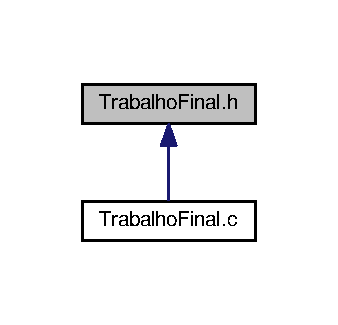
\includegraphics[width=162pt]{TrabalhoFinal_8h__dep__incl}
\end{center}
\end{figure}
\subsection*{Functions}
\begin{DoxyCompactItemize}
\item 
void \hyperlink{TrabalhoFinal_8h_a38e4a81c795cc1492e2dbf4388dc2e03}{keyboard\+Func} (unsigned char key, int x, int y)
\begin{DoxyCompactList}\small\item\em Funcionalidades do teclado, onde todas as funcionalidades e animações do programa serão feitas pelo teclado. As funcionalidades estão listadas em detalha na página inical da documentação. \end{DoxyCompactList}\item 
void \hyperlink{TrabalhoFinal_8h_a503dca08df7da12b8659d41ed3fdf9fa}{rot\+Key\+Func} (int key, int x, int y)
\begin{DoxyCompactList}\small\item\em Trata as quatro possibilidades de movimentos rotacionais (cima,baixo,esquerda,direita). \end{DoxyCompactList}\item 
void \hyperlink{TrabalhoFinal_8h_aa0bf20c41c51e3378eff1bed8c8ad7e7}{Key\+Up} ()
\begin{DoxyCompactList}\small\item\em As quatro funções\+: Key\+Up, Key\+Down, Key\+Left e Key\+Right limitam a mudança de direção de rotação apenas com \char`\"{}reset\char`\"{}. \end{DoxyCompactList}\item 
void \hyperlink{TrabalhoFinal_8h_a67b12319ab360702a47400465268d886}{Key\+Down} ()
\begin{DoxyCompactList}\small\item\em As quatro funções\+: Key\+Up, Key\+Down, Key\+Left e Key\+Right limitam a mudança de direção de rotação apenas com \char`\"{}reset\char`\"{}. \end{DoxyCompactList}\item 
void \hyperlink{TrabalhoFinal_8h_a8feed104082b0773ee6a1e43dc62494a}{Key\+Left} ()
\begin{DoxyCompactList}\small\item\em As quatro funções\+: Key\+Up, Key\+Down, Key\+Left e Key\+Right limitam a mudança de direção de rotação apenas com \char`\"{}reset\char`\"{}. \end{DoxyCompactList}\item 
void \hyperlink{TrabalhoFinal_8h_a247cd4807e203e488d19c3e2d11d0dfe}{Key\+Right} ()
\begin{DoxyCompactList}\small\item\em As quatro funções\+: Key\+Up, Key\+Down, Key\+Left e Key\+Right limitam a mudança de direção de rotação apenas com \char`\"{}reset\char`\"{}. \end{DoxyCompactList}\item 
void \hyperlink{TrabalhoFinal_8h_a0a8efd509aaffafefd6d761748e3b688}{Reset\+Animation} ()
\begin{DoxyCompactList}\small\item\em Restaura posição original e define rotação igual a zero. \end{DoxyCompactList}\item 
void \hyperlink{TrabalhoFinal_8h_aaad754c5c3683cfa1ff97d2c381f7cf9}{Zero\+Rotation} ()
\begin{DoxyCompactList}\small\item\em Restaura posicao original e define rotação igual a zero. \end{DoxyCompactList}\item 
void \hyperlink{TrabalhoFinal_8h_acdf384c0ffd8a916ef177390d4231f20}{Shade\+Model\+Func} ()
\begin{DoxyCompactList}\small\item\em Sombra, alterna entre G\+L\+\_\+\+S\+M\+O\+O\+T\+H e G\+L\+\_\+\+F\+L\+A\+T. \end{DoxyCompactList}\item 
void \hyperlink{TrabalhoFinal_8h_a6d5b5815603b85d7b4c4cbcef41c9d04}{Fill\+Model\+Func} ()
\begin{DoxyCompactList}\small\item\em Preenchimento do poligono, alterna entre G\+L\+\_\+\+L\+I\+N\+E e G\+L\+\_\+\+F\+I\+L\+L. \end{DoxyCompactList}\item 
void \hyperlink{TrabalhoFinal_8h_a49231a37c9b57e3f5985645eea705aea}{Inc\+U} ()
\begin{DoxyCompactList}\small\item\em Incrementa \char`\"{}u\char`\"{}. \end{DoxyCompactList}\item 
void \hyperlink{TrabalhoFinal_8h_a9a94b4a40c2579e84929e96cd020fc76}{Dec\+U} ()
\begin{DoxyCompactList}\small\item\em Decrementa \char`\"{}u\char`\"{}. \end{DoxyCompactList}\item 
void \hyperlink{TrabalhoFinal_8h_a382fd47ad46d351c01316369a7a2a167}{Inc\+V} ()
\begin{DoxyCompactList}\small\item\em Incrementa \char`\"{}u\char`\"{}. \end{DoxyCompactList}\item 
void \hyperlink{TrabalhoFinal_8h_a243cc6a279207dca01da3d7e00f6a669}{Dec\+V} ()
\begin{DoxyCompactList}\small\item\em Decrementa \char`\"{}u\char`\"{}. \end{DoxyCompactList}\item 
void \hyperlink{TrabalhoFinal_8h_a5b0721aa50b4ff19c67311b6d8717635}{update\+Scene} (void)
\begin{DoxyCompactList}\small\item\em Desenha superfícies/retalhos com todas suas especificações. \end{DoxyCompactList}\item 
void \hyperlink{TrabalhoFinal_8h_a17a53fe9e683b81bdc7618f88b8b8502}{init\+Rendering} ()
\begin{DoxyCompactList}\small\item\em Inicializa Open\+G\+L (iluminação). \end{DoxyCompactList}\item 
void \hyperlink{TrabalhoFinal_8h_a5228d95579d96f983dea42fed8845620}{resize\+Window} (int w, int h)
\begin{DoxyCompactList}\small\item\em Efetua mudança nas dimensões da janela (aumentando ou diminuindo de acordo com ação do mouse). \end{DoxyCompactList}\end{DoxyCompactItemize}


\subsection{Detailed Description}
Declaração das funções para o programa Trabalho\+Final. 

\begin{DoxyAuthor}{Author}
Grupo (ordem alfabética)\+: Igor, Nathália \& Yves 
\end{DoxyAuthor}


\subsection{Function Documentation}
\hypertarget{TrabalhoFinal_8h_a9a94b4a40c2579e84929e96cd020fc76}{\index{Trabalho\+Final.\+h@{Trabalho\+Final.\+h}!Dec\+U@{Dec\+U}}
\index{Dec\+U@{Dec\+U}!Trabalho\+Final.\+h@{Trabalho\+Final.\+h}}
\subsubsection[{Dec\+U}]{\setlength{\rightskip}{0pt plus 5cm}void Dec\+U (
\begin{DoxyParamCaption}
{}
\end{DoxyParamCaption}
)}}\label{TrabalhoFinal_8h_a9a94b4a40c2579e84929e96cd020fc76}


Decrementa \char`\"{}u\char`\"{}. 

\begin{DoxyReturn}{Returns}
Void 
\end{DoxyReturn}
\hypertarget{TrabalhoFinal_8h_a243cc6a279207dca01da3d7e00f6a669}{\index{Trabalho\+Final.\+h@{Trabalho\+Final.\+h}!Dec\+V@{Dec\+V}}
\index{Dec\+V@{Dec\+V}!Trabalho\+Final.\+h@{Trabalho\+Final.\+h}}
\subsubsection[{Dec\+V}]{\setlength{\rightskip}{0pt plus 5cm}void Dec\+V (
\begin{DoxyParamCaption}
{}
\end{DoxyParamCaption}
)}}\label{TrabalhoFinal_8h_a243cc6a279207dca01da3d7e00f6a669}


Decrementa \char`\"{}u\char`\"{}. 

\begin{DoxyReturn}{Returns}
Void 
\end{DoxyReturn}
\hypertarget{TrabalhoFinal_8h_a6d5b5815603b85d7b4c4cbcef41c9d04}{\index{Trabalho\+Final.\+h@{Trabalho\+Final.\+h}!Fill\+Model\+Func@{Fill\+Model\+Func}}
\index{Fill\+Model\+Func@{Fill\+Model\+Func}!Trabalho\+Final.\+h@{Trabalho\+Final.\+h}}
\subsubsection[{Fill\+Model\+Func}]{\setlength{\rightskip}{0pt plus 5cm}void Fill\+Model\+Func (
\begin{DoxyParamCaption}
{}
\end{DoxyParamCaption}
)}}\label{TrabalhoFinal_8h_a6d5b5815603b85d7b4c4cbcef41c9d04}


Preenchimento do poligono, alterna entre G\+L\+\_\+\+L\+I\+N\+E e G\+L\+\_\+\+F\+I\+L\+L. 

\begin{DoxyReturn}{Returns}
Void 
\end{DoxyReturn}
\hypertarget{TrabalhoFinal_8h_a49231a37c9b57e3f5985645eea705aea}{\index{Trabalho\+Final.\+h@{Trabalho\+Final.\+h}!Inc\+U@{Inc\+U}}
\index{Inc\+U@{Inc\+U}!Trabalho\+Final.\+h@{Trabalho\+Final.\+h}}
\subsubsection[{Inc\+U}]{\setlength{\rightskip}{0pt plus 5cm}void Inc\+U (
\begin{DoxyParamCaption}
{}
\end{DoxyParamCaption}
)}}\label{TrabalhoFinal_8h_a49231a37c9b57e3f5985645eea705aea}


Incrementa \char`\"{}u\char`\"{}. 

\begin{DoxyReturn}{Returns}
Void 
\end{DoxyReturn}
\hypertarget{TrabalhoFinal_8h_a382fd47ad46d351c01316369a7a2a167}{\index{Trabalho\+Final.\+h@{Trabalho\+Final.\+h}!Inc\+V@{Inc\+V}}
\index{Inc\+V@{Inc\+V}!Trabalho\+Final.\+h@{Trabalho\+Final.\+h}}
\subsubsection[{Inc\+V}]{\setlength{\rightskip}{0pt plus 5cm}void Inc\+V (
\begin{DoxyParamCaption}
{}
\end{DoxyParamCaption}
)}}\label{TrabalhoFinal_8h_a382fd47ad46d351c01316369a7a2a167}


Incrementa \char`\"{}u\char`\"{}. 

\begin{DoxyReturn}{Returns}
Void 
\end{DoxyReturn}
\hypertarget{TrabalhoFinal_8h_a17a53fe9e683b81bdc7618f88b8b8502}{\index{Trabalho\+Final.\+h@{Trabalho\+Final.\+h}!init\+Rendering@{init\+Rendering}}
\index{init\+Rendering@{init\+Rendering}!Trabalho\+Final.\+h@{Trabalho\+Final.\+h}}
\subsubsection[{init\+Rendering}]{\setlength{\rightskip}{0pt plus 5cm}void init\+Rendering (
\begin{DoxyParamCaption}
{}
\end{DoxyParamCaption}
)}}\label{TrabalhoFinal_8h_a17a53fe9e683b81bdc7618f88b8b8502}


Inicializa Open\+G\+L (iluminação). 

\begin{DoxyReturn}{Returns}
Void 
\end{DoxyReturn}
\hypertarget{TrabalhoFinal_8h_a38e4a81c795cc1492e2dbf4388dc2e03}{\index{Trabalho\+Final.\+h@{Trabalho\+Final.\+h}!keyboard\+Func@{keyboard\+Func}}
\index{keyboard\+Func@{keyboard\+Func}!Trabalho\+Final.\+h@{Trabalho\+Final.\+h}}
\subsubsection[{keyboard\+Func}]{\setlength{\rightskip}{0pt plus 5cm}void keyboard\+Func (
\begin{DoxyParamCaption}
\item[{unsigned char}]{key, }
\item[{int}]{x, }
\item[{int}]{y}
\end{DoxyParamCaption}
)}}\label{TrabalhoFinal_8h_a38e4a81c795cc1492e2dbf4388dc2e03}


Funcionalidades do teclado, onde todas as funcionalidades e animações do programa serão feitas pelo teclado. As funcionalidades estão listadas em detalha na página inical da documentação. 


\begin{DoxyParams}{Parameters}
{\em key} & tecla pressionada pelo usuário \\
\hline
{\em x} & coordenada x do ponto atual \\
\hline
{\em y} & coordenada y do ponto atual \\
\hline
\end{DoxyParams}
\begin{DoxyReturn}{Returns}
Void 
\end{DoxyReturn}
\hypertarget{TrabalhoFinal_8h_a67b12319ab360702a47400465268d886}{\index{Trabalho\+Final.\+h@{Trabalho\+Final.\+h}!Key\+Down@{Key\+Down}}
\index{Key\+Down@{Key\+Down}!Trabalho\+Final.\+h@{Trabalho\+Final.\+h}}
\subsubsection[{Key\+Down}]{\setlength{\rightskip}{0pt plus 5cm}void Key\+Down (
\begin{DoxyParamCaption}
{}
\end{DoxyParamCaption}
)}}\label{TrabalhoFinal_8h_a67b12319ab360702a47400465268d886}


As quatro funções\+: Key\+Up, Key\+Down, Key\+Left e Key\+Right limitam a mudança de direção de rotação apenas com \char`\"{}reset\char`\"{}. 

\begin{DoxyReturn}{Returns}
Void 
\end{DoxyReturn}
\hypertarget{TrabalhoFinal_8h_a8feed104082b0773ee6a1e43dc62494a}{\index{Trabalho\+Final.\+h@{Trabalho\+Final.\+h}!Key\+Left@{Key\+Left}}
\index{Key\+Left@{Key\+Left}!Trabalho\+Final.\+h@{Trabalho\+Final.\+h}}
\subsubsection[{Key\+Left}]{\setlength{\rightskip}{0pt plus 5cm}void Key\+Left (
\begin{DoxyParamCaption}
{}
\end{DoxyParamCaption}
)}}\label{TrabalhoFinal_8h_a8feed104082b0773ee6a1e43dc62494a}


As quatro funções\+: Key\+Up, Key\+Down, Key\+Left e Key\+Right limitam a mudança de direção de rotação apenas com \char`\"{}reset\char`\"{}. 

\begin{DoxyReturn}{Returns}
Void 
\end{DoxyReturn}
\hypertarget{TrabalhoFinal_8h_a247cd4807e203e488d19c3e2d11d0dfe}{\index{Trabalho\+Final.\+h@{Trabalho\+Final.\+h}!Key\+Right@{Key\+Right}}
\index{Key\+Right@{Key\+Right}!Trabalho\+Final.\+h@{Trabalho\+Final.\+h}}
\subsubsection[{Key\+Right}]{\setlength{\rightskip}{0pt plus 5cm}void Key\+Right (
\begin{DoxyParamCaption}
{}
\end{DoxyParamCaption}
)}}\label{TrabalhoFinal_8h_a247cd4807e203e488d19c3e2d11d0dfe}


As quatro funções\+: Key\+Up, Key\+Down, Key\+Left e Key\+Right limitam a mudança de direção de rotação apenas com \char`\"{}reset\char`\"{}. 

\begin{DoxyReturn}{Returns}
Void 
\end{DoxyReturn}
\hypertarget{TrabalhoFinal_8h_aa0bf20c41c51e3378eff1bed8c8ad7e7}{\index{Trabalho\+Final.\+h@{Trabalho\+Final.\+h}!Key\+Up@{Key\+Up}}
\index{Key\+Up@{Key\+Up}!Trabalho\+Final.\+h@{Trabalho\+Final.\+h}}
\subsubsection[{Key\+Up}]{\setlength{\rightskip}{0pt plus 5cm}void Key\+Up (
\begin{DoxyParamCaption}
{}
\end{DoxyParamCaption}
)}}\label{TrabalhoFinal_8h_aa0bf20c41c51e3378eff1bed8c8ad7e7}


As quatro funções\+: Key\+Up, Key\+Down, Key\+Left e Key\+Right limitam a mudança de direção de rotação apenas com \char`\"{}reset\char`\"{}. 

\begin{DoxyReturn}{Returns}
Void 
\end{DoxyReturn}
\hypertarget{TrabalhoFinal_8h_a0a8efd509aaffafefd6d761748e3b688}{\index{Trabalho\+Final.\+h@{Trabalho\+Final.\+h}!Reset\+Animation@{Reset\+Animation}}
\index{Reset\+Animation@{Reset\+Animation}!Trabalho\+Final.\+h@{Trabalho\+Final.\+h}}
\subsubsection[{Reset\+Animation}]{\setlength{\rightskip}{0pt plus 5cm}void Reset\+Animation (
\begin{DoxyParamCaption}
{}
\end{DoxyParamCaption}
)}}\label{TrabalhoFinal_8h_a0a8efd509aaffafefd6d761748e3b688}


Restaura posição original e define rotação igual a zero. 

\begin{DoxyReturn}{Returns}
Void 
\end{DoxyReturn}
\hypertarget{TrabalhoFinal_8h_a5228d95579d96f983dea42fed8845620}{\index{Trabalho\+Final.\+h@{Trabalho\+Final.\+h}!resize\+Window@{resize\+Window}}
\index{resize\+Window@{resize\+Window}!Trabalho\+Final.\+h@{Trabalho\+Final.\+h}}
\subsubsection[{resize\+Window}]{\setlength{\rightskip}{0pt plus 5cm}void resize\+Window (
\begin{DoxyParamCaption}
\item[{int}]{w, }
\item[{int}]{h}
\end{DoxyParamCaption}
)}}\label{TrabalhoFinal_8h_a5228d95579d96f983dea42fed8845620}


Efetua mudança nas dimensões da janela (aumentando ou diminuindo de acordo com ação do mouse). 


\begin{DoxyParams}{Parameters}
{\em w} & tamanho da largura da janela \\
\hline
{\em h} & tamanho altura da janela \\
\hline
\end{DoxyParams}
\begin{DoxyReturn}{Returns}
Void 
\end{DoxyReturn}
\hypertarget{TrabalhoFinal_8h_a503dca08df7da12b8659d41ed3fdf9fa}{\index{Trabalho\+Final.\+h@{Trabalho\+Final.\+h}!rot\+Key\+Func@{rot\+Key\+Func}}
\index{rot\+Key\+Func@{rot\+Key\+Func}!Trabalho\+Final.\+h@{Trabalho\+Final.\+h}}
\subsubsection[{rot\+Key\+Func}]{\setlength{\rightskip}{0pt plus 5cm}void rot\+Key\+Func (
\begin{DoxyParamCaption}
\item[{int}]{key, }
\item[{int}]{x, }
\item[{int}]{y}
\end{DoxyParamCaption}
)}}\label{TrabalhoFinal_8h_a503dca08df7da12b8659d41ed3fdf9fa}


Trata as quatro possibilidades de movimentos rotacionais (cima,baixo,esquerda,direita). 


\begin{DoxyParams}{Parameters}
{\em key} & tecla pressionada pelo usuário \\
\hline
{\em x} & coordenada x do ponto atual \\
\hline
{\em y} & coordenada y do ponto atual \\
\hline
\end{DoxyParams}
\begin{DoxyReturn}{Returns}
Void 
\end{DoxyReturn}
\hypertarget{TrabalhoFinal_8h_acdf384c0ffd8a916ef177390d4231f20}{\index{Trabalho\+Final.\+h@{Trabalho\+Final.\+h}!Shade\+Model\+Func@{Shade\+Model\+Func}}
\index{Shade\+Model\+Func@{Shade\+Model\+Func}!Trabalho\+Final.\+h@{Trabalho\+Final.\+h}}
\subsubsection[{Shade\+Model\+Func}]{\setlength{\rightskip}{0pt plus 5cm}void Shade\+Model\+Func (
\begin{DoxyParamCaption}
{}
\end{DoxyParamCaption}
)}}\label{TrabalhoFinal_8h_acdf384c0ffd8a916ef177390d4231f20}


Sombra, alterna entre G\+L\+\_\+\+S\+M\+O\+O\+T\+H e G\+L\+\_\+\+F\+L\+A\+T. 

\begin{DoxyReturn}{Returns}
Void 
\end{DoxyReturn}
\hypertarget{TrabalhoFinal_8h_a5b0721aa50b4ff19c67311b6d8717635}{\index{Trabalho\+Final.\+h@{Trabalho\+Final.\+h}!update\+Scene@{update\+Scene}}
\index{update\+Scene@{update\+Scene}!Trabalho\+Final.\+h@{Trabalho\+Final.\+h}}
\subsubsection[{update\+Scene}]{\setlength{\rightskip}{0pt plus 5cm}void update\+Scene (
\begin{DoxyParamCaption}
\item[{void}]{}
\end{DoxyParamCaption}
)}}\label{TrabalhoFinal_8h_a5b0721aa50b4ff19c67311b6d8717635}


Desenha superfícies/retalhos com todas suas especificações. 

\begin{DoxyReturn}{Returns}
Void 
\end{DoxyReturn}
\hypertarget{TrabalhoFinal_8h_aaad754c5c3683cfa1ff97d2c381f7cf9}{\index{Trabalho\+Final.\+h@{Trabalho\+Final.\+h}!Zero\+Rotation@{Zero\+Rotation}}
\index{Zero\+Rotation@{Zero\+Rotation}!Trabalho\+Final.\+h@{Trabalho\+Final.\+h}}
\subsubsection[{Zero\+Rotation}]{\setlength{\rightskip}{0pt plus 5cm}void Zero\+Rotation (
\begin{DoxyParamCaption}
{}
\end{DoxyParamCaption}
)}}\label{TrabalhoFinal_8h_aaad754c5c3683cfa1ff97d2c381f7cf9}


Restaura posicao original e define rotação igual a zero. 

\begin{DoxyReturn}{Returns}
Void 
\end{DoxyReturn}

%--- End generated contents ---

% Index
\newpage
\phantomsection
\addcontentsline{toc}{chapter}{Index}
\printindex

\end{document}
